\documentclass[amssymb,twocolumn,aps]{revtex4}

% allows special characters (including æøå)
\usepackage[utf8]{inputenc}
%\usepackage [norsk]{babel} %if you write norwegian
\usepackage[english]{babel}  %if you write english

\usepackage{physics,amssymb}  % mathematical symbols (physics imports amsmath)
\usepackage{graphicx}         % include graphics such as plots
\graphicspath{{../figures}}  % set the path for figures
\usepackage{xcolor}           % set colors
\usepackage{hyperref}         % automagic cross-referencing 
\usepackage{float}			  % force placement of tables and figures
\hypersetup{hidelinks}        % hide link colors

\begin{document}
\title{Polynomial Regression on Runge's Function\\
    \normalsize FYS-STK3155 - Project 1}
\date{October 5, 2026}
\author{Hassen M. Morad}
\affiliation{Honours Student, University of Oslo}
\email{hmmorad@student.matnat.uio.no}

\newpage

\begin{abstract}
    Polynomial regression provides a simple way to study the bias-variance trade-off as model complexity increases. High-degree polynomials can reduce bias, but simultaneously increase variance and lead to overfitting, making model selection important. We studied this behaviour using polynomials up to degree 15 for Runge's function $f(x) = \frac{1}{1+25x^2}$ on $[-1,1]$, with $n=100$ samples and Gaussian noise with standard deviation $\sigma=0.1$. We used OLS, Ridge and Lasso regression, together with bootstrap resampling and $k$-fold cross-validation, and compared the closed-form estimators with our own implementations of gradient descent, momentum, AdaGrad, RMSProp, Adam, and stochastic gradient descent. Cross-validation selected OLS at degree 10 (test $R^2=0.70$), while Ridge and Lasso selected degree 6 and reached test $R^2=0.74$ and $0.81$, respectively. Momentum converged fastest to the closed-form solution once tuned. Our results show how resampling can be used to compare models, regularization can reduce overfitting, and the choice of optimizer affects convergence.
\end{abstract}

\maketitle

\section{Introduction}
When we fit a model, we want it to capture the relationship in the data, without fitting the noise in the observations. A model with low complexity can be too simple to describe the data, while a more complex model can become sensitive to the training set and perform poorly on new observations. Finding the right balance is important.

Runge's function is a classic example that illustrates this problem. While the function itself is simple and smooth, polynomials of high degree can develop large oscillations near the boundaries of the interval. This shows how increasing the complexity of a model does not automatically lead to better predictions, and motivates the use of regularization and resampling methods when selecting a model.

We first fit polynomial models using OLS and Ridge regression and study how the test error changes with polynomial degree, and for Ridge, the regularization parameter. We also fit with Lasso regression and examine how the $\ell_1$ penalty affects the fitted coefficients. OLS estimates the coefficients by minimizing the squared residuals, while Ridge adds an $\ell_2$ penalty that shrinks the coefficients towards zero. Lasso instead uses an $\ell_1$ penalty, which can shrink individual coefficients exactly to zero \cite{hastie}.

We implemented all three models ourselves using NumPy\cite{numpy}, including forming the design matrices, parameter estimation, and regularization terms. We split the data into training and test sets using Scikit-learn's \texttt{train\_test\_split()} function \cite{scikit-learn}.

To determine which models generalize well, we need a way to evaluate them beyond a single training set. We therefore use resampling methods to investigate both model performance and the bias-variance trade-off, with the available data. In $k$-fold cross-validation, the data are divided into $k$ folds, with each fold used once as validation set, while the model is fitted to the remaining folds \cite{hastie}. We use this to compare different polynomial degrees and choose the regularization parameter $\lambda$ for Ridge and Lasso.

Bootstrap resampling instead generates multiple training sets by sampling with replacement, and refits the model to each sample. This allows the variation in predictions across the samples to be used to study bias and variance \cite{hastie}. The bootstrap procedure and bias-variance calculations were implemented by us, where we used Scikit-learn's \texttt{resample()} function. $k$-fold cross-validation was performed using \texttt{Kfold()} from Scikit-learn \cite{scikit-learn}.

We also investigate how the model parameters can be found using iterative optimization methods. For OLS and Ridge, the parameters can be obtained directly using closed-form solutions, which provides a reference for evaluating the iterative methods. Lasso does not have a closed-form solution because of its $\ell_1$ penalty, making iterative optimization necessary. We compare gradient descent, momentum, AdaGrad, RMSProp, Adam, and stochastic gradient descent. These methods use the gradient of the cost function to update the parameters iteratively, but differ in how the updates and learning rates are calculated \cite{lecturebook}.

We implemented the optimization algorithms and their update rules ourselves. The gradients were derived analytically and also computed using automatic differentiation with JAX \cite{jax}.

Section \ref{section:methods} presents the models and the bias-variance decomposition. Section \ref{section:Implementation} describes our implementation and the tests against the closed-form solutions, and Section \ref{section:results} presents the results with discussion, first for OLS, then Ridge and Lasso, then the optimisers. In Section \ref{section:conclusion} we conclude our findings. The code is available at \url{https://github.com/hmmorad/FYS-STK3155-Project1}.


\section{Methods}\label{section:methods}
\subsection{Regression Models}
\subsubsection{Ordinary Least Squares (OLS)}

Given observations $(x_i,y_i)$, we fit a polynomial of degree $m-1$,
\[
    p(x) = \sum_{j=1}^{m} \theta_j x^{j-1} = \theta_1 + \theta_2x + \theta_3x^2 + \cdots + \theta_mx^{m-1}
\]
For observations $y_1,\ldots,y_n$, the coefficients can be found by minimizing
\[
    \sum_{i=1}^{n} \left(p(x_i)-y_i\right)^2.
\]
This can be written as the matrix least squares problem
\[
    \min_{\boldsymbol{\theta}} \|\boldsymbol{X}\mathbf{\boldsymbol{\theta}}-\mathbf{\boldsymbol{y}}\|_2^2,
\]
where
\[
    \boldsymbol{\theta}=
    \begin{bmatrix}
        \theta_1 & \theta_2 & \cdots & \theta_m
    \end{bmatrix}^T,
    \qquad
    \mathbf{\boldsymbol{y}}
    =
    \begin{bmatrix}
        y_1 & y_2 & \cdots & y_n
    \end{bmatrix}^T,
\]
and $\boldsymbol{X}$ is the Vandermonde matrix:
\[
    \boldsymbol{X} =
    \begin{bmatrix}
        1      & x_1    & x_1^2  & \cdots & x_1^{m-1} \\
        1      & x_2    & x_2^2  & \cdots & x_2^{m-1} \\
        \vdots & \vdots & \vdots &        & \vdots    \\
        1      & x_n    & x_n^2  & \cdots & x_n^{m-1}
    \end{bmatrix}.
\]
OLS finds the coefficients by minimizing the mean squared error. Differentiating with respect to $\boldsymbol{\theta}$ gives
\[
    \nabla C_{\mathrm{OLS}}(\boldsymbol{\theta})
    =
    \frac{2}{n}\boldsymbol{X}^T(\boldsymbol{X}\boldsymbol{\theta}-\mathbf{\boldsymbol{y}}).
\]
Setting the gradient to zero gives the normal equations, and when $\boldsymbol{X}^T\boldsymbol{X}$ is invertible,
\begin{equation}
    \hat{\boldsymbol{\theta}}_{\mathrm{OLS}}
    =
    (\boldsymbol{X}^T\boldsymbol{X})^{-1}\boldsymbol{X}^T\mathbf{\boldsymbol{y}}.
    \label{eq}
\end{equation}

As the polynomial degree increases, the columns of $\boldsymbol{X}$ can become highly correlated, making the problem poorly conditioned. We therefore use the singular value decomposition (SVD) rather than forming $\boldsymbol{X}^T\boldsymbol{X}$, which makes the conditioning worse. Writing

\[
    \boldsymbol{X}=U\Sigma V^T.
\]
and substituting it into the normal equations, it can be shown \cite{lecturebook} that this is equivalent with
\begin{equation}
    \hat{\boldsymbol{\theta}}_{\mathrm{OLS}}
    =
    \sum_i
    \frac{u_i^T\mathbf{\boldsymbol{y}}}{\sigma_i}v_i.
    \label{eq:ols_svd_sum}
\end{equation}
This also shows why small singular values can be problematic. Since $u_i^T\mathbf y$ is divided by $\sigma_i$, small changes in the data can lead to large changes in the coefficients when $\sigma_i$ is small.

\subsubsection{Ridge}
Ridge regression reduces this sensitivity by adding an $\ell_2$ penalty to the OLS cost,
\begin{equation}
    C_{\mathrm{Ridge}}(\boldsymbol{\theta})
    =
    \frac{1}{n}\|\boldsymbol{X}\boldsymbol{\theta}-\mathbf{\boldsymbol{y}}\|_2^2
    +\lambda\|\boldsymbol{\theta}\|_2^2,
    \label{eq:ridge_cost}
\end{equation}
where $\lambda \geq 0$ controls the strength of the regularization penalty.
Differentiating with respect to $\boldsymbol{\theta}$ gives
\[
    \nabla C_{\mathrm{Ridge}}(\boldsymbol{\theta})
    =
    \frac{2}{n}\boldsymbol{X}^T(\boldsymbol{X}{\boldsymbol{\theta}}-\mathbf{\boldsymbol{y}})
    +2\lambda{\boldsymbol{\theta}},
\]
and therefore
\begin{equation}
    \hat{\boldsymbol{\theta}}_{\mathrm{Ridge}}
    =
    (\boldsymbol{X}^T\boldsymbol{X}+n\lambda \boldsymbol{I})^{-1}\boldsymbol{X}^T\mathbf{\boldsymbol{y}}.
    \label{eq:ridge}
\end{equation}
Using the SVD of $\boldsymbol{X}$, it can be shown that \cite{lecturebook}
\begin{equation}
    \hat{\boldsymbol{\theta}}_{\mathrm{Ridge}}
    =
    \sum_i
    \frac{\sigma_i}
    {\sigma_i^2+n\lambda}
    (u_i^T\mathbf{\boldsymbol{y}})v_i.
    \label{eq:ridge_svd}
\end{equation}
This can be compared with the OLS solution in Eq.~\eqref{eq:ols_svd_sum}, where the corresponding factor is $1/\sigma_i$. For Ridge, this factor becomes
\[
    \frac{\sigma_i}{\sigma_i^2+n\lambda}
    =
    \frac{1}{\sigma_i}
    \frac{\sigma_i^2}{\sigma_i^2+n\lambda}.
\]

The second factor is between zero and one, so Ridge reduces the contribution from each direction. The reduction is strongest for small singular values \cite{lecturebook}.

\subsubsection{Lasso}
Lasso regression replaces the $\ell_2$ penalty with an $\ell_1$ penalty,
\[
    C_{\mathrm{Lasso}}(\boldsymbol{\theta})
    =
    \frac{1}{n}\|\boldsymbol{X}\boldsymbol{\theta}-\mathbf{\boldsymbol{y}}\|_2^2
    +\lambda\|\boldsymbol{\theta}\|_1.
\]
The absolute value is not differentiable at zero, so Lasso does not have a closed-form solution like OLS and Ridge. Instead, it is fitted using iterative optimization methods. For $\theta_j\neq0$, the derivative of $|\theta_j|$ is $\operatorname{sign}(\theta_j)$, while at $\theta_j=0$ any value in $[-1,1]$ is a valid subgradient \cite{lecturebook}. Therefore, apart from zero, the Lasso subgradient is
\begin{equation}
    \nabla C_{\mathrm{Lasso}}(\boldsymbol{\theta})
    =
    \frac{2}{n}\boldsymbol{X}^T
    (\boldsymbol{X}\boldsymbol{\theta}-\mathbf{\boldsymbol{y}})
    +
    \lambda\,\operatorname{sign}(\boldsymbol{\theta}), \label{eq:gradient_lasso}
\end{equation}
with a valid choice of subgradient used when a coefficient is zero \cite{lecturebook}.

\subsection{The bias-variance decomposition}

To study the bias-variance tradeoff, we consider the noisy model $y=f(x)+\varepsilon,$
where $\mathbb{E}[\varepsilon]=0$ and $\operatorname{Var}(\varepsilon)=\sigma^2$. For a fixed test point $x$, let $\tilde y$ be the prediction from a model trained on a randomly drawn training set. We start with the expected squared error and add and subtract $\mathbb{E}[\tilde{y}]$ inside of it,
\[
    \mathbb{E}\left[(y-\tilde{y})^2\right]
    =
    \mathbb{E}\left[
        \left(
        \left(y-\mathbb{E}[\tilde{y}]\right)
        -
        \left(\tilde{y}-\mathbb{E}[\tilde{y}]\right)
        \right)^2
        \right].
\]
Expanding the square with $(a-b)^2=a^2-2ab+b^2$ splits this into three terms
\[
    \begin{aligned}
        \mathbb{E}\left[(y-\tilde{y})^2\right]
        ={} &
        \underbrace{\mathbb{E}\left[\left(y-\mathbb{E}[\tilde{y}]\right)^2\right]}_{\text{Term A}}                                                   \\
            & \underbrace{-2\mathbb{E}\left[\left(y-\mathbb{E}[\tilde{y}]\right)\left(\tilde{y}-\mathbb{E}[\tilde{y}]\right)\right]}_{\text{Term B}} \\
            & +
        \underbrace{\mathbb{E}\left[\left(\tilde{y}-\mathbb{E}[\tilde{y}]\right)^2\right]}_{\text{Term C}}.
    \end{aligned}
\]
Inserting $y=f(x)+\varepsilon$ into Term A gives
\begin{equation}
    \begin{aligned}
        \text{Term A}
         & =
        \mathbb{E}\left[
            \left(f(x)-\mathbb{E}[\tilde{y}]+\varepsilon\right)^2
        \right] \\
         & =
        \left(f(x)-\mathbb{E}[\tilde{y}]\right)^2
        +\sigma^2,
    \end{aligned}
    \label{eq:term_a}
\end{equation}
since the cross term vanishes because $f(x)-\mathbb{E}[\tilde{y}]$ is a fixed number ($f$ is non-stochastic) and $\mathbb{E}[\varepsilon]=0$ (zero-mean noise). The first part of Eq.~\eqref{eq:term_a} is the squared bias.

Term B, after the same substitution, splits into two pieces,
\[
    \begin{aligned}
        \text{Term B}
        ={} &
        -2\mathbb{E}\left[
            \left(f(x)-\mathbb{E}[\tilde{y}]\right)
            \left(\tilde{y}-\mathbb{E}[\tilde{y}]\right)
        \right]                  \\
            & -2\mathbb{E}\left[
            \varepsilon\left(\tilde{y}-\mathbb{E}[\tilde{y}]\right)
            \right].
    \end{aligned}
\]

The first piece is zero because $f(x)-\mathbb{E}[\tilde{y}]$ is a fixed number that can be moved outside the expectation, leaving $\mathbb{E}[\tilde{y}]-\mathbb{E}[\tilde{y}]=0$. The second piece is zero because the test noise $\varepsilon$ is independent of the training data, and $\tilde{y}$ is the prediction from a model fitted on that training data. Hence, $\varepsilon$ and $\tilde{y}$ are independent, giving $\mathbb{E}[\varepsilon(\tilde{y}-\mathbb{E}[\tilde{y}])]=\mathbb{E}[\varepsilon]\,\mathbb{E}[\tilde{y}-\mathbb{E}[\tilde{y}]]=0$ (using that we have zero-mean noise). Term B therefore vanishes entirely.

Term C is simply the variance, $\operatorname{Var}(\tilde{y})$. Collecting Terms A and C, with Term B equalling to zero, gives the bias-variance decomposition,
\begin{equation}
    \mathbb{E}\left[(y-\tilde{y})^2\right]
    =
    \underbrace{
        \left(f(x)-\mathbb{E}[\tilde{y}]\right)^2
    }_{\text{bias}^2}
    +
    \underbrace{
        \operatorname{Var}(\tilde{y})
    }_{\text{variance}}
    +
    \underbrace{\sigma^2}_{\text{noise}}.
    \label{eq:bias_variance}
\end{equation}

The bias measures how far the average prediction is from the true function, while the variance measures how much the prediction changes when the training set changes. The noise term represents the irreducible uncertainty in the observations.

Since the true function $f$ is known in this project, we can calculate the theoretical bias directly. However in practice, $f(x)$ is unknown, so we use the noisy test observations $y=f(x)+\varepsilon$ to estimate the bias. For a set of test observations, the empirical average is therefore
\[
    \frac{1}{n}\sum_{i=1}^n
    \left(y_{i}-\mathbb{E}[\tilde{y}_i]\right)^2.
\]
This is the same quantity as inside Term A, averaged over the test observations. As $n$ increases, by the law of large numbers, this average approaches its expectation. Therefore, by Eq.~\eqref{eq:term_a}, its expectation is
\[
    \left(f_i-\mathbb{E}[\tilde{y}_i]\right)^2+\sigma^2.
\]
Therefore,
\[
    \text{estimated bias}^2
    =
    \text{true bias}^2+\sigma^2.
\]

The estimated bias is larger than the true squared bias because it also contains the irreducible noise.

\subsection{Gradient-Based Optimization}\label{subsection:gradient}

We use iterative optimization for Lasso, and also use it as an alternative to the closed-form solutions for OLS and Ridge. Using the gradients, gradient descent updates the parameters according to
\begin{equation}
    \boldsymbol{\theta}_{t+1}
    =
    \boldsymbol{\theta}_t
    -
    \gamma\nabla C(\boldsymbol{\theta}_t),
    \label{eq:gradient_descent}
\end{equation}
where $\gamma$ is the learning rate and $t=0,1,2,\ldots$ is the iteration.

The Hessians of the OLS and Ridge costs are
\[
    H_{\mathrm{OLS}}
    =
    \frac{2}{n}X^TX
\]
and
\[
    H_{\mathrm{Ridge}}
    =
    \frac{2}{n}X^TX+2\lambda I.
\]
For gradient descent to converge, it can be shown that the learning rate must satisfy
\[
    0<\gamma<\frac{2}{\lambda_{\max}}
    :=\gamma_{\max},
\]
where $\lambda_{\max}$ is the largest eigenvalue of the Hessian. The learning rate giving the theoretically fastest convergence is
\[
    \gamma^*
    =
    \frac{2}{\lambda_{\min}+\lambda_{\max}},
\]
where $\lambda_{\min}$ is the smallest eigenvalue \cite{lecturebook}.

Momentum modifies gradient descent by using information from previous gradients, which can accelerate the convergence,
\[
    \boldsymbol{v}_t = \beta\boldsymbol{v}_{t-1} + \gamma\nabla C(\boldsymbol{\theta}_t),
    \qquad
    \boldsymbol{\theta}_{t+1} = \boldsymbol{\theta}_t - \boldsymbol{v}_t,
\]
where $\beta$ controls the contribution from previous updates.
Like plain gradient descent, momentum uses the same learning rate $\gamma$ for all parameters. The adaptive methods instead adjust the learning rate for each parameter based on the size of its previous gradients. A parameter with consistently large gradients receives smaller updates, while a parameter with smaller gradients can receive larger updates \cite{lecturebook}.

Let $g_t:=\nabla C(\theta_t)$ be the gradient at step $t$. AdaGrad accumulates the sum of squared gradients, $r_t=r_{t-1}+g_t^2$ with $r_0=0$, and updates
\[
    \theta_{t+1} = \theta_t - \frac{\gamma}{\sqrt{r_t+\epsilon}}\,g_t,
\]
coordinate by coordinate (where $\epsilon$ is a small constant that prevents division by zero). As more gradients are accumulated, $r_t$ grows, so the step sizes become smaller over time.

RMSProp instead uses an exponentially weighted average,
\[
    r_t=\rho r_{t-1}+(1-\rho)g_t^2,
\]
so that recent gradients have more influence and the step sizes do not continually decrease.

Adam combines a moving average of the gradients (like in momentum) with the squared-gradient estimate used by RMSProp,
\[
    m_t = \beta_1 m_{t-1} + (1-\beta_1)g_t,
    \qquad
    r_t = \beta_2 r_{t-1} + (1-\beta_2)g_t^2,
\]
with $m_0=r_0=0$. Both averages are initially biased towards zero because they start from zero. Adam removes this bias by dividing by the factors $1-\beta_1^t$ and $1-\beta_2^t$ before updating the parameters,
\[
    \theta_{t+1} = \theta_t - \gamma\,
    \frac{m_t/(1-\beta_1^t)}{\sqrt{r_t/(1-\beta_2^t)}+\epsilon}.
\]

\subsection{Stochastic Gradient Descent (SGD)}
Stochastic gradient descent (SGD) approximates the full gradient using a mini-batch $\mathcal{B}$ of size $M$ drawn from the training data. For OLS, the mini-batch gradient is
\[
    \nabla C_{\mathcal{B}}(\boldsymbol{\theta})
    =
    \frac{2}{M}\sum_{i\in\mathcal{B}}\boldsymbol{x}_i\left(\boldsymbol{x}_i^T\boldsymbol{\theta}-y_i\right).
\]
At the start of each epoch, the training data are reshuffled and divided into mini-batches. The mini-batch gradient can be used with any of the optimization algorithms described in section~\ref{subsection:gradient}. Since the mini-batch gradient is only an estimate of the full gradient, the updates contain noise. The standard deviation decreases approximately as $1/\sqrt{M}$ \cite{lecturebook}, so larger batches give more accurate but more (computationally) expensive gradient estimates, while smaller batches give cheaper but noisier updates.

With a constant learning rate, this noise remains, even as the parameters approach the minimum. SGD therefore fluctuates around the minimum rather than converging to it exactly. A decaying learning rate can be used to reduce the effect \cite{lecturebook}.

\subsection{Automatic differentiation}
Symbolic differentiation suffers from expression swells and numerical differentiation suffers from truncation errors, which automatic differentiation avoids. Instead, it uses the chain rule along the evaluation trace and computational graph to calculate the numerical, exact value of the derivative at a given point \cite{lecturebook}.

By the Cheap Gradient Principle, reverse-mode automatic differentiation can compute both $f(\boldsymbol{x})$ and the complete gradient $\nabla f(\boldsymbol{x})$ in at most $c,l$ operations, where $l$ is the number of operations required to evaluate $f$ and $c\leq4$ is a constant. Automatic differentiation is therefore useful where deriving a symbolic expression is almost computationally impossible \cite{lecturebook}.


\section{Implementation}\label{section:Implementation}

We implemented the project as a small Python package, using separate classes for models, optimizers, and resampling. \texttt{OLS}, \texttt{Ridge}, and \texttt{Lasso} inherit from a \texttt{BaseModel} class, which contains the design matrix, target values, parameters, and cost and gradient calculations. OLS and Ridge have a \texttt{closed\_form()} function that finds the coefficients using the SVD we derived in Section~\ref{section:methods}. The gradient of the cost function is implemented analytically, with \texttt{np.sign()} used for the $\ell_1$ penalty in Lasso. The cost function is also implemented using JAX, which allows its gradient to be calculated with automatic differentiation.

The optimizers inherit from a common \texttt{Optimizer} class. Each optimizer implements its own \texttt{step()} and \texttt{reset()} method, while the common \texttt{optimize()} method handles the optimization loop.

The \texttt{ModelFitter} class is a simple interface that takes in a \texttt{model\_class} and an optional \texttt{Optimizer}. Its \texttt{fit()} method creates the model and uses its closed-form solution when no optimizer is provided. Otherwise, the model is passed to the optimizer. For example, OLS can be fitted using its closed-form solution:

{\footnotesize
\begin{verbatim}
fitter = ModelFitter(OLS)
model = fitter.fit(X, y)
\end{verbatim}
}

The same interface can also be used with an optimizer:

{\footnotesize
\begin{verbatim}
fitter = ModelFitter(OLS, optimizer=GradientDescent())
model = fitter.fit(X, y)
\end{verbatim}
}

\texttt{ModelFitter} is also used by the \texttt{Bootstrap} and \texttt{CrossValidation} classes, which allows the resampling code to be used with different models and fitting methods. The bootstrap uses Scikit-learn's \texttt{resample()} function, while cross-validation uses \texttt{KFold}.

The data were split into training and test sets using Scikit-learn's \texttt{train\_test\_split()}, with 80\% used for training and 20\% for testing. The polynomial features were standardized using the mean and standard deviation of the training data, while the target values were centered by subtracting the training mean. The intercept was therefore not included in the design matrix. When making predictions, the training mean is added back to the model output, so the predictions are on the original target scale.

Scaling is important for Ridge and Lasso, since the regularization terms depend on the magnitude of the coefficients. Without scaling, polynomial features with different scales would be penalized differently. Scaling also improves the conditioning of the design matrix. The scaling parameters were fitted only on the training data and then applied to the test data. The same process was used within each cross-validation fold to avoid data leakage from the validation data \cite{lecturebook}.

Analytical gradients were compared with gradients obtained using JAX, and the gradient-based OLS and Ridge solutions were compared with their closed-form solutions. The Lasso implementation was compared with Scikit-learn's \texttt{Lasso}. The project notebook was also used to run the bootstrap, cross-validation, and SGD experiments and to produce the figures and tables presented in the results in Section~\ref{section:results}.

\section{Results and Discussion}\label{section:results}

Unless stated otherwise, the results use $N=100$ samples from Runge's function on $[-1,1]$, with Gaussian noise $\sigma=0.1$ and an $80/20$ train-test split. The random seed was fixed to 2026.

\subsection{Ordinary least squares}

\begin{figure}[htbp]
    \centering
    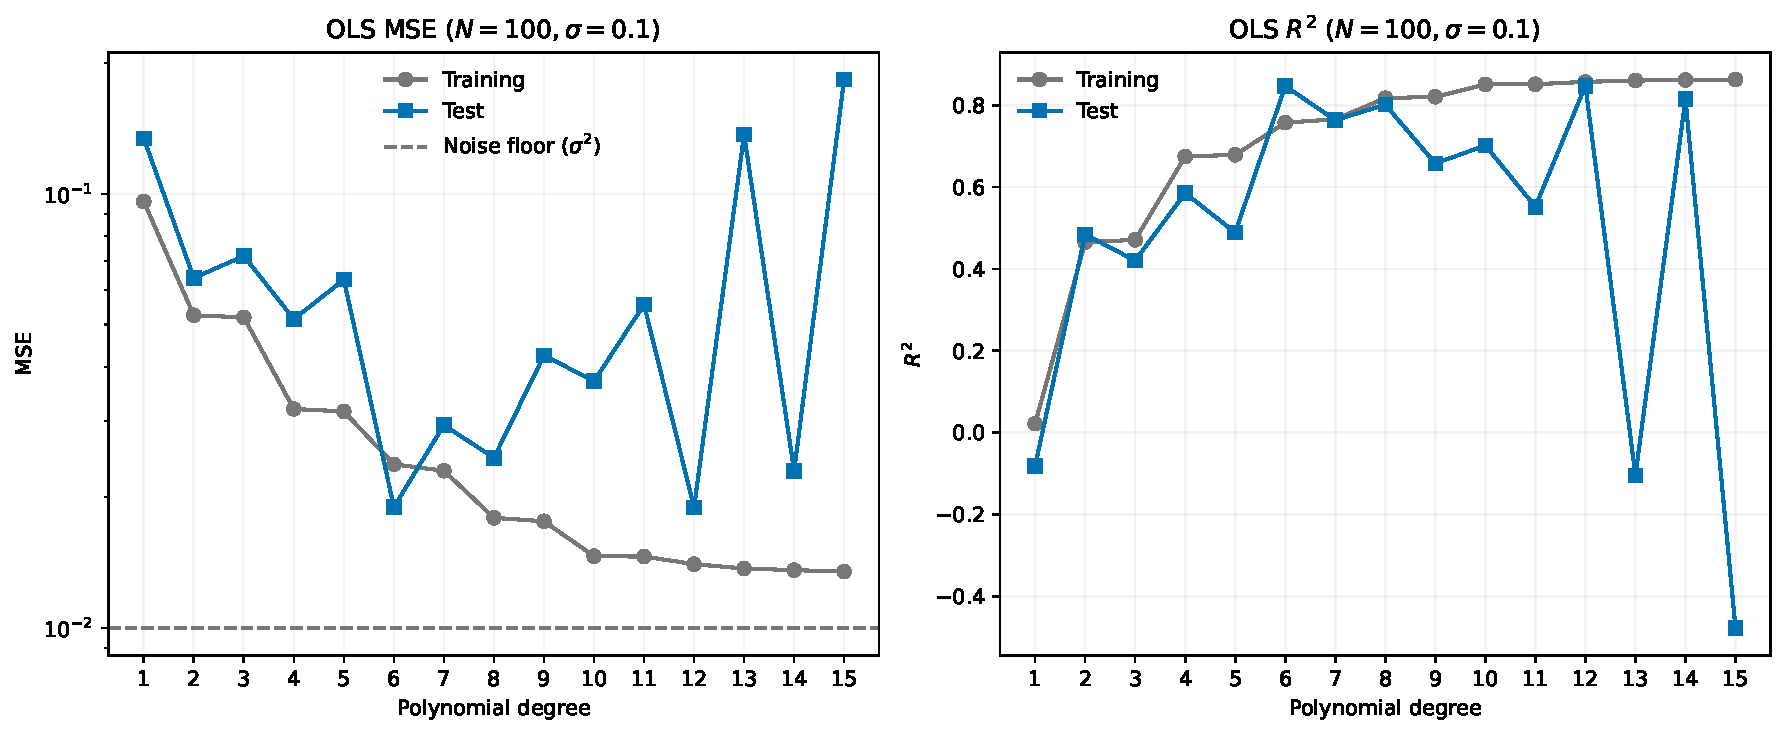
\includegraphics[width=\linewidth]{part_a_ols_mse_r2.pdf}
    \caption{OLS training and test MSE (left) and $R^2$ (right) as functions of polynomial degree, for $N=100$ and $\sigma=0.1$. The dashed line marks the noise floor $\sigma^2$.}
    \label{fig:part_a_mse_r2}
\end{figure}

Figure~\ref{fig:part_a_mse_r2} shows the effect of increasing the polynomial degree. The training MSE decreases as the degree increases, since the model has more flexibility to fit the training data. On the other hand, the test MSE first decreases and then increases. At higher degrees, the test MSE fluctuates because the fitted coefficients become more sensitive to the particular training sample, but the overall increase in test error is clear. The lowest test MSE is obtained at degree 12 with a test $R^2$ of approximately $0.8473$, while degree 6 gives a very similar test $R^2$ of approximately $0.8469$. Increasing the degree further does not seem improve the test error and eventually makes it worse, with $R^2\approx -0.5$ for degree 15, meaning that the model performs worse than simply predicting the mean.

\begin{table}[htbp]
    \centering
    \caption{OLS sensitivity to noise level and sample size.}
    \label{tab:ols-sensitivity}
\begin{tabular}{rrrrrr}
\hline\hline
N & $\sigma$ & Best degree & Train MSE & Test MSE & Test $R^2$ \\
\hline
100 & 0.1 & 12 & 0.01403 & 0.01894 & 0.8473 \\
100 & 0.3 & 7 & 0.1354 & 0.1106 & 0.5686 \\
100 & 0.5 & 7 & 0.3597 & 0.3011 & 0.3523 \\
100 & 0.1 & 12 & 0.01403 & 0.01894 & 0.8473 \\
300 & 0.1 & 13 & 0.01145 & 0.01367 & 0.7843 \\
500 & 0.1 & 15 & 0.009648 & 0.01439 & 0.8541 \\
\hline\hline
\end{tabular}
\end{table}


The effect of the noise level and sample size is shown in Table~\ref{tab:ols-sensitivity}. Increasing the noise from $\sigma=0.1$ to $\sigma=0.5$ reduces the best test $R^2$ from $0.847$ to $0.352$, while the degree giving the lowest test error decreases from 12 to 7. With more noise, fitting the higher-order behaviour becomes less useful because the additional flexibility also makes the fitted model more sensitive to the noise in the training data. Increasing the sample size from $N=100$ to $N=500$, while keeping the noise level fixed at $\sigma=0.1$, has the opposite effect. The best degrees increases for both, with the best degree for $N=500$ going to 15, which is the largest degree tested, and without a loss in $R^2$.

With more observations, the higher degree fits become less sensitive to the particular training sample, since the dataset is larger and provides more information about the underlying function. This reduces the variation caused by random differences in the training data, which makes it possible to use higher-degree models.

\begin{figure}[htbp]
    \centering
    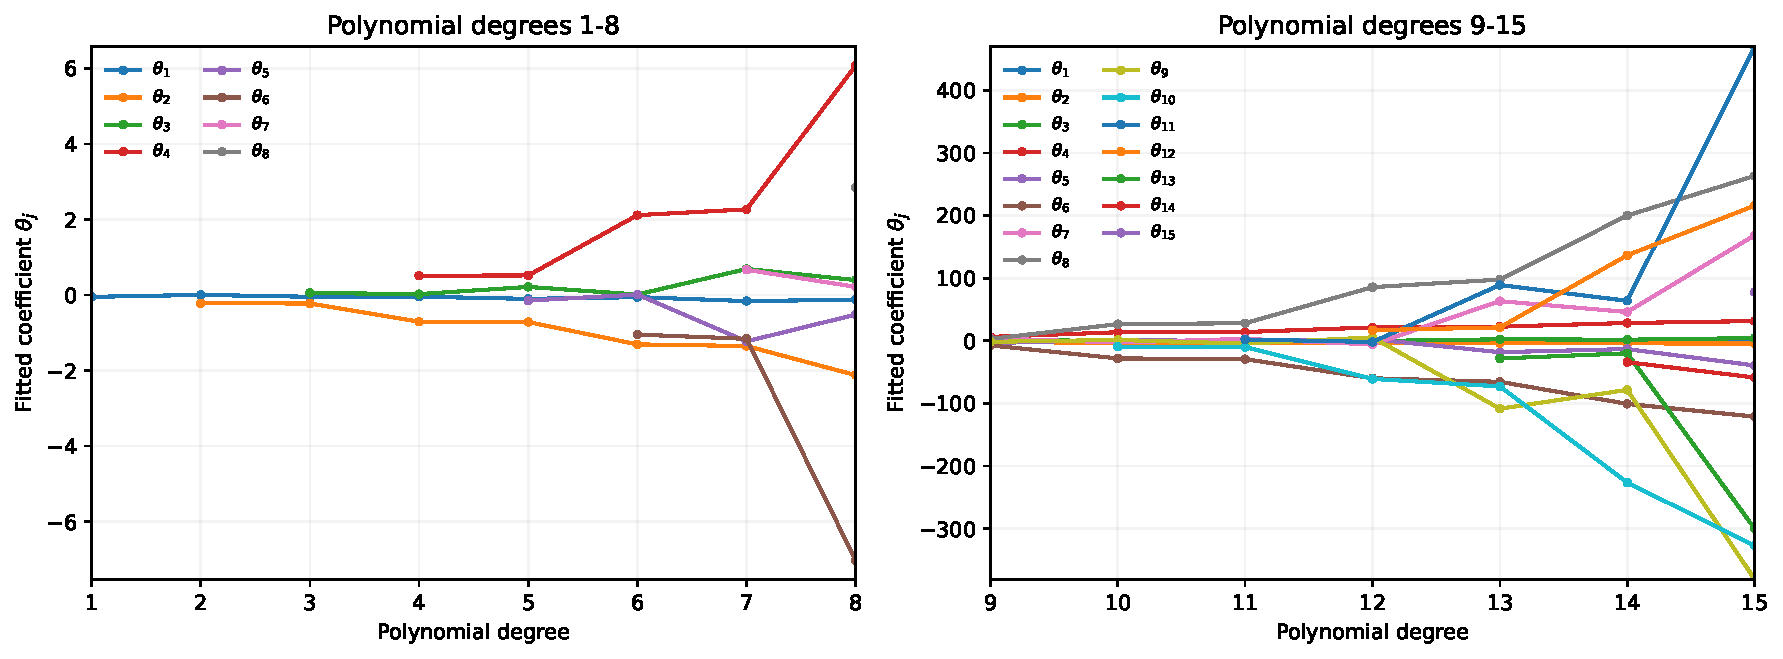
\includegraphics[width=\linewidth]{part_a_ols_theta.pdf}
    \caption{Fitted OLS coefficients $\theta_j$ as a function of polynomial degree, split into two panels for readability. $N=100$ and $\sigma=0.1$.}
    \label{fig:part_a_theta}
\end{figure}

\begin{figure}[htbp]
    \centering
    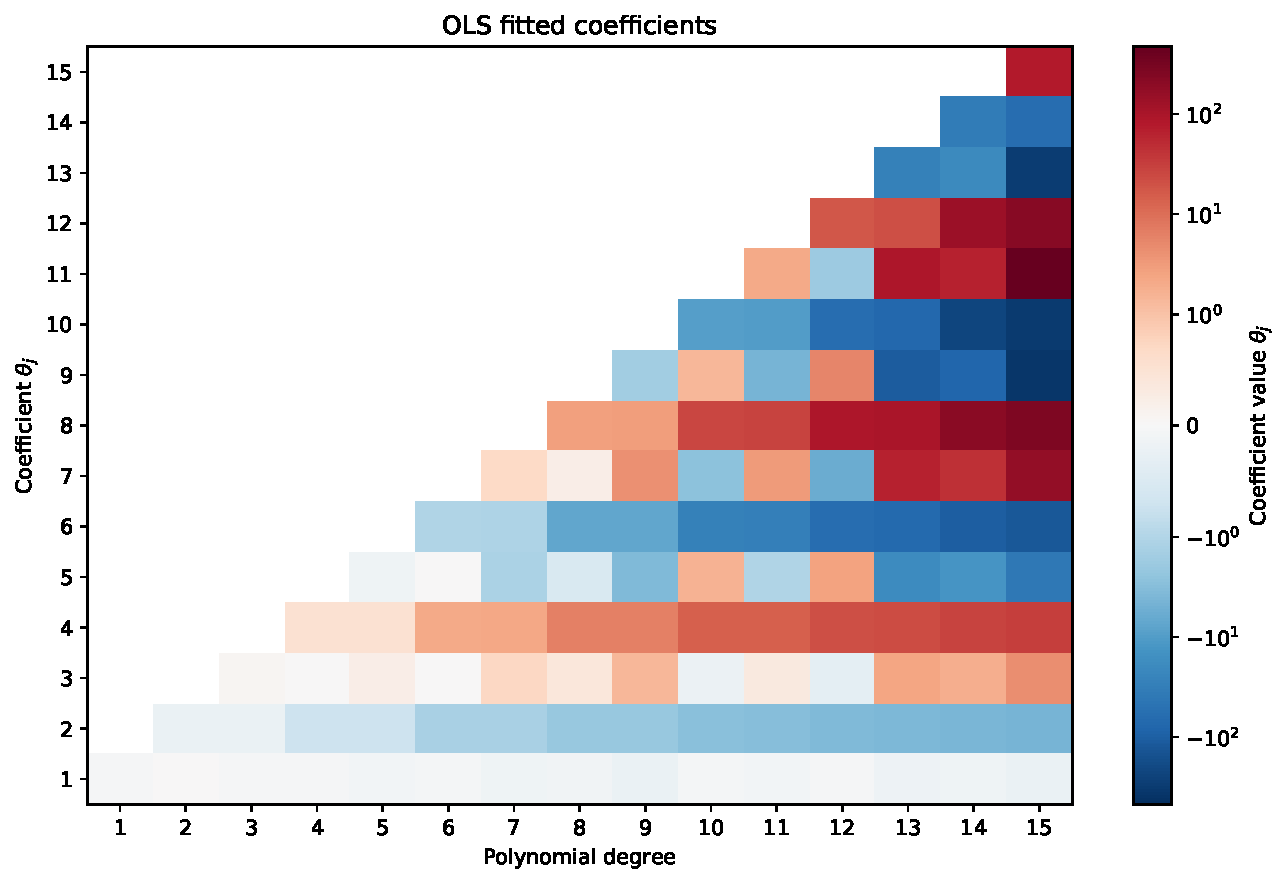
\includegraphics[width=\linewidth]{part_a_ols_theta_heatmap.pdf}
    \caption{Heatmap of the fitted OLS coefficients $\theta_j$ as a function of polynomial degree. $N=100$ and $\sigma=0.1$.}
    \label{fig:part_a_theta_heatmap}
\end{figure}

Figures~\ref{fig:part_a_theta} and~\ref{fig:part_a_theta_heatmap} show the fitted coefficients, for $N=100$ and $\sigma=0.1$. For low degrees the coefficients are small and stable, but from around degree 10, the coefficients become very large and alternate in sign. The resulting polynomial model we end up with can still give a reasonable prediction, because these terms partly cancel each other, but the fitted parameters become sensitive to the data. This can be explained by the small singular values discussed in Section~\ref{section:methods}. The design matrix develops near-collinear columns, so when the OLS solution in Eq.~\eqref{eq:ols_svd_sum} divides by small singular values $\sigma_i$, it can result into large, oscillating coefficients.

This also illustrates why the degree-12 result we found for $N=100$ and $\sigma=0.1$, should not be interpreted as the final model choice. The degree was selected here by looking at the test error, which means that the test set is being used for model selection. Later, we use cross-validation on the training data to make this choice without using the test set.


\subsection{Ridge regression}

\begin{figure}[htbp]
    \centering
    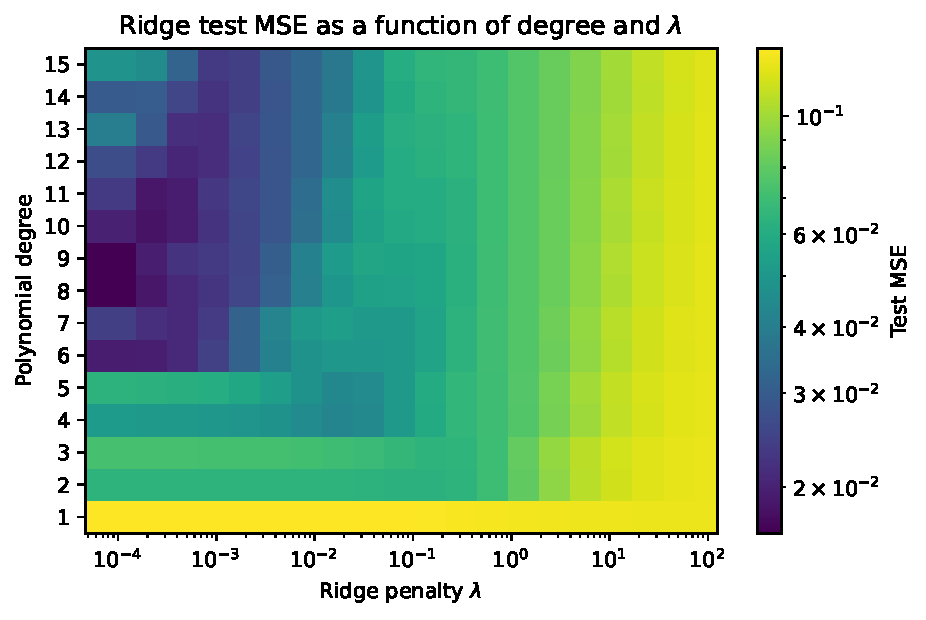
\includegraphics[width=\linewidth]{part_b_ridge_test_mse_heatmap.pdf}
    \caption{Ridge test MSE as a function of polynomial degree and regularization strength $\lambda$ (logarithmic color scale).}
    \label{fig:part_b_heatmap}
\end{figure}


Figure~\ref{fig:part_b_heatmap} shows the full degree-$\lambda$ grid. From the colors, we see that as the polynomial degree increases, we tend to get a lower test MSE for small $\lambda$, and that the range of about degree 6-12 seem to have the same test MSE. For larger $\lambda$, the test MSE becomes less dependent on the polynomial degree, so a wider range of degrees gives similar results.

This can be explained by the SVD solution in Eq.~\eqref{eq:ridge_svd}. Higher-degree polynomials introduce additional components with small singular values, which are the components that made the OLS solution sensitive to small changes in the training data. The Ridge penalty shrinks these components more strongly as $\lambda$ increases. As a result, the additional high-degree components have less influence on the fitted model, so increasing the polynomial degree has a smaller effect on the test MSE.

\begin{figure}[htbp]
    \centering
    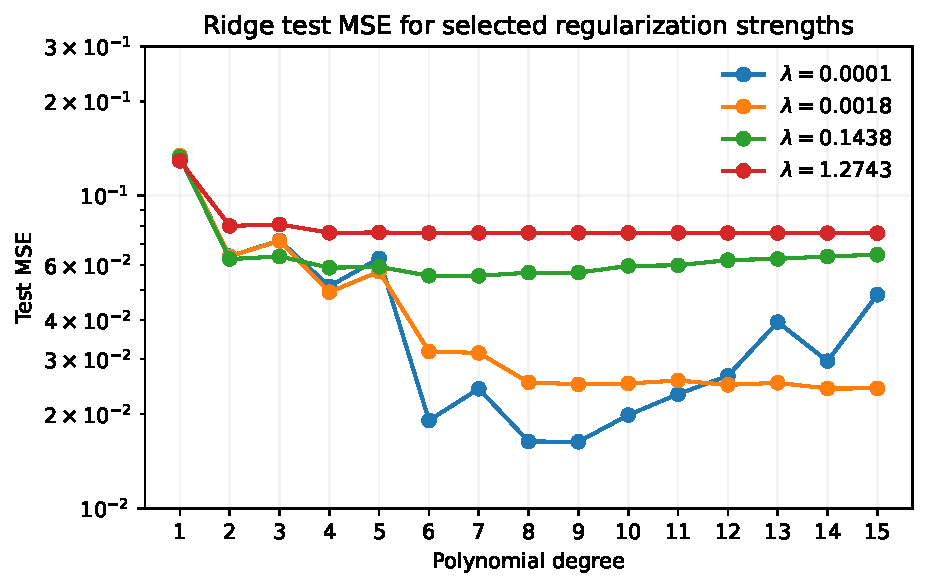
\includegraphics[width=\linewidth]{part_b_ridge_selected_lambda.pdf}
    \caption{Ridge test MSE as a function of polynomial degree for four selected values of $\lambda$.}
    \label{fig:part_b_curves}
\end{figure}

Figure~\ref{fig:part_b_curves} shows this more clearly. With the smallest $\lambda$, the test MSE still increases a bit at higher degrees, giving a similar curve to OLS (typical U-shape). For the other values of $\lambda$, a wider range of polynomial degrees gives similar test MSE, and the curves become extremely flat.  However, at the intermediate degrees (around 6-10), the smallest $\lambda$ still gives the lowest test MSE, while larger $\lambda$ values give slightly higher errors.


\subsection{The bias-variance trade-off and the bootstrap}

\begin{figure}[htbp]
    \centering
    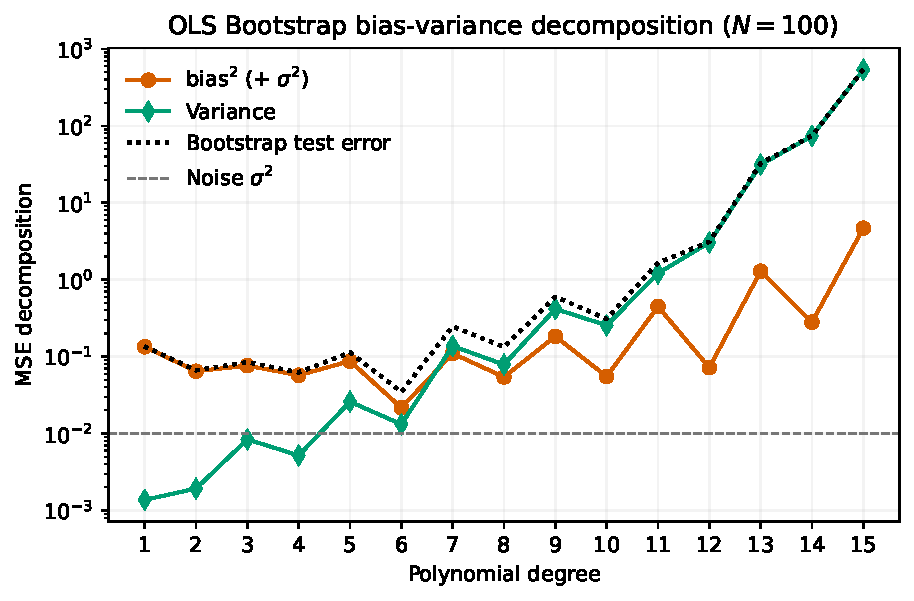
\includegraphics[width=\linewidth]{part_c_bootstrap_bias_variance.pdf}
    \caption{Bootstrap estimate of the (measured) bias$^2$, variance and total test error for OLS, as a function of polynomial degree ($N=100$, 1000 bootstrap samples).}
    \label{fig:part_c_bias_variance}
\end{figure}

Figure~\ref{fig:part_c_bias_variance} reproduces the decomposition of Eq.~\eqref{eq:bias_variance}, and gives a more direct view of why the test error changes with degree. At low degree the error is dominated by bias: the polynomial is too simple to follow Runge's function, and resampling the training data does not change it. As the degree increases: the bias decreases and the variance increases. Around degrees 7-8, the variance starts to dominate the error, which is consistent with the large, unstable coefficients seen in Figure.~\ref{fig:part_a_theta}. The total bootstrap error therefore has a minimum between the bias-dominated region at low degrees and the  variance-dominated region at high degrees.

\begin{figure}[htbp]
    \centering
    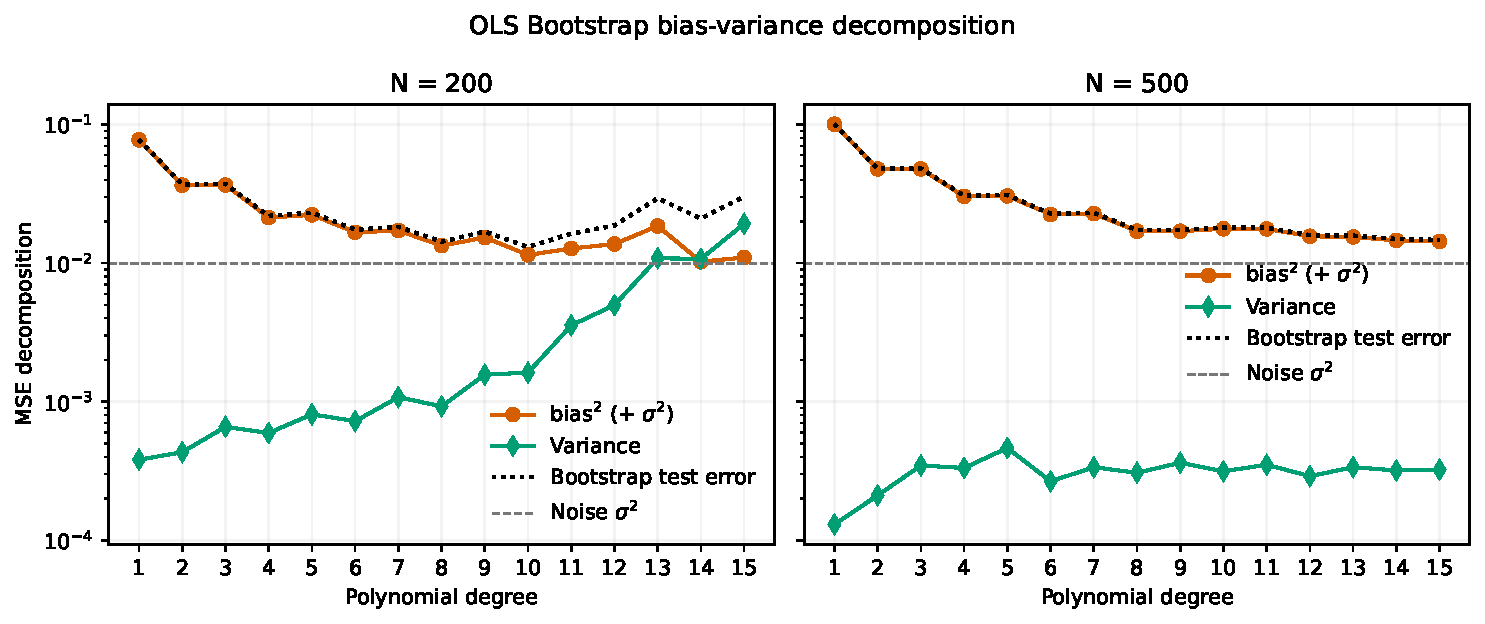
\includegraphics[width=\linewidth]{part_c_sample_size_comparison.pdf}
    \caption{The same bootstrap bias-variance decomposition at $N=200$ and $N=500$.}
    \label{fig:part_c_sample_size}
\end{figure}

Figure~\ref{fig:part_c_sample_size} shows what happens with more data. The bias curve changes very little from $N=100$ in Figure~\ref{fig:part_c_bias_variance}, because it is the polynomial degree that determines how well a model can approximate the true function $f$.  The bias measures how far the average prediction is from the true function, and increasing the amount of data does not change the true function or the polynomial degrees being fitted. However, the variance curve drops as $N$ increases, since each bootstrap sample then better represents the full training distribution. This agrees with the OLS sensitivity results in Table~\ref{tab:ols-sensitivity}, where $N=500$ allowed a degree of 15.

The increase in variance at higher polynomial degrees can be addressed by regularization. The penalty discourages large coefficients, making the fitted model less sensitive to changes in the training data and therefore reduces the variance. For Ridge regression, it can be shown that increasing the penalty increases bias while decreasing variance \cite{lecturebook}. Regularization therefore trades variance for bias.

\subsection{Cross-validation}

\begin{figure}[htbp]
    \centering
    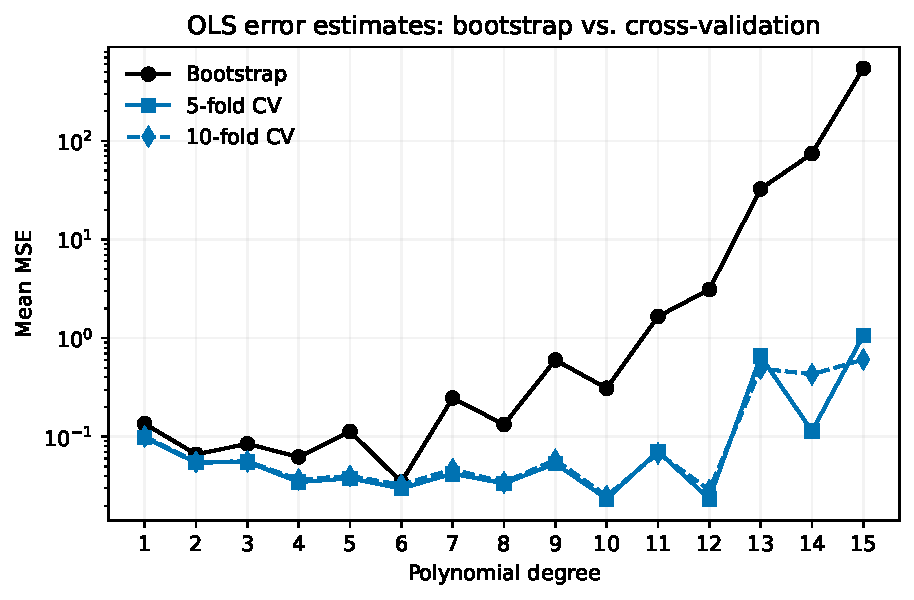
\includegraphics[width=\linewidth]{part_d_ols_cv_vs_bootstrap.pdf}
    \caption{OLS error estimates from the bootstrap, 5-fold and 10-fold cross-validation.}
    \label{fig:part_d_ols}
\end{figure}

Figure~\ref{fig:part_d_ols} compares the bootstrap test error from Fig.~\ref{fig:part_c_bias_variance} with 5-fold and 10-fold cross-validation. We see that the 5-fold and 10-fold cross-validation curves are essentially identical, with only degree 14 and 15 being slightly different. As for the errors between the bootstrap and cross-validation, we see that they agree on lower degrees, but the bootstrap error starts to rise more quickly from degree 7, and become noticeably larger at the highest degrees.

One possible reason is the effective training-set size in each resample. A bootstrap sample contains $N$ draws, but because the sampling is done with replacement, only about $63.2\%$ of the original observations are unique on average \cite{hastie}. The effective training set for the bootstrap is therefore smaller than for cross-validation, which can explain why the bootstrap error rises more quickly at higher degrees. In Figure~\ref{fig:part_c_sample_size}, we see that increasing $N$ reduces the variance, since the model is fitted using more observations and is therefore less sensitive to random differences in the training data.

\begin{figure}[htbp]
    \centering
    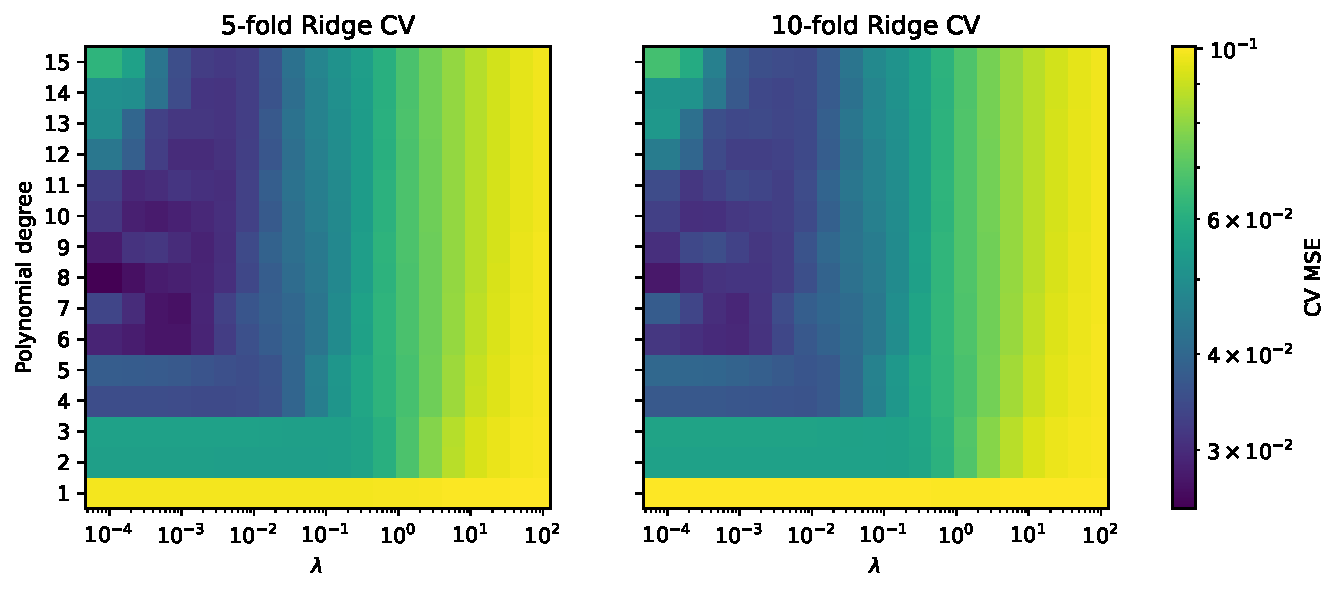
\includegraphics[width=\linewidth]{part_d_ridge_cv_heatmaps.pdf}
    \caption{5-fold and 10-fold cross-validated Ridge MSE as a function of degree and $\lambda$.}
    \label{fig:part_d_ridge}
\end{figure}

Figure~\ref{fig:part_d_ridge} shows the cross-validation results for Ridge. We also note here that there is almost no difference between 5-fold and 10-fold cross-validation. Comparing the CV results with the test MSE in Figure~\ref{fig:part_b_heatmap}, we see a similar overall pattern, with polynomial degrees around 4-12 giving low errors for small $\lambda$. However, the CV results show the low errors over a wider range of $\lambda$ values, from $10^{-4}$ to $10^{-1}$.

The lowest 10-fold CV MSE is found at degree 8 and $\lambda=10^{-4}$. However, for the final comparison, we use the one-standard-error rule rather than simply choosing the lowest CV error.

\subsection{Gradient descent and automatic differentiation}

Before using gradient descent, we checked our analytical gradients against JAX's automatic differentiation at a random $\boldsymbol{\theta}$. We found that the maximum absolute difference was $2.7\times10^{-15}$ for both OLS and Ridge, and therefore agree to machine precision.

\begin{figure}[htbp]
    \centering
    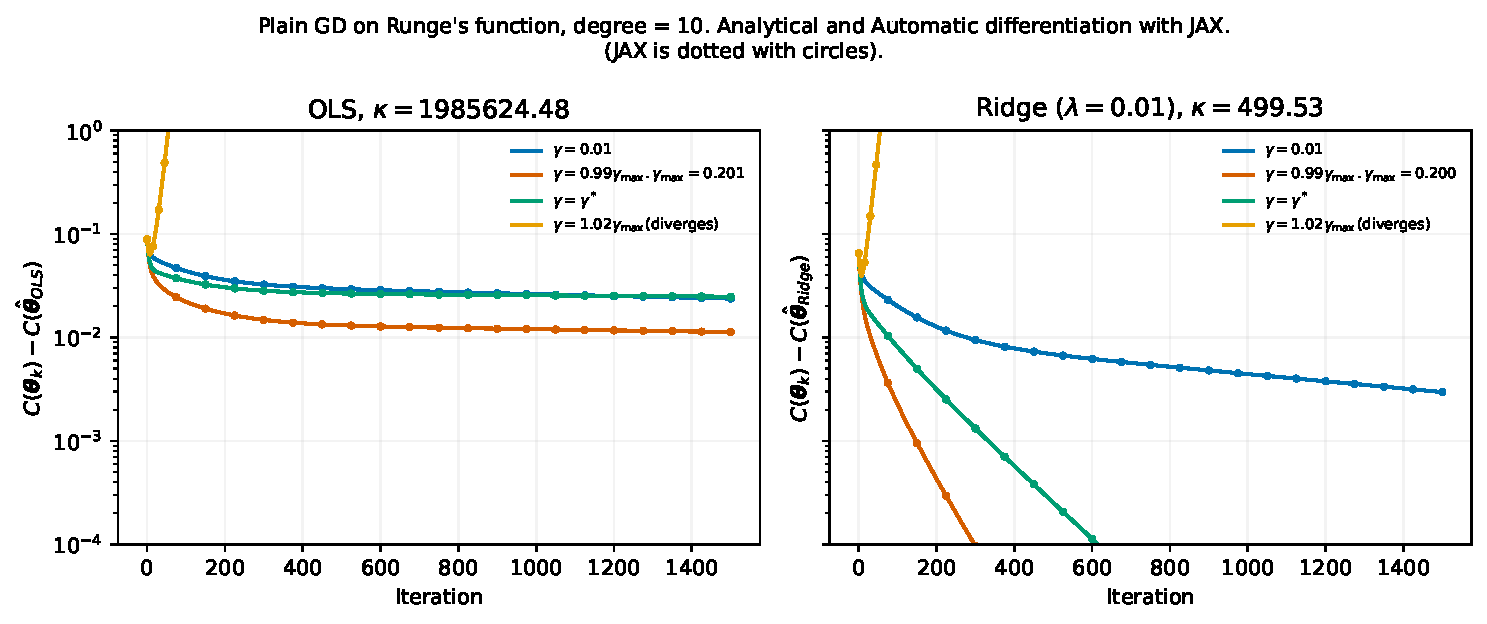
\includegraphics[width=\linewidth]{part_e_gd_distance_to_closed_form.pdf}
    \caption{Excess cost of plain gradient descent for degree-10, OLS and Ridge ($\lambda=0.01$), for several learning rates $\gamma$. JAX gradients (dotted circles) and analytical gradients (continuous lines) overlap.}
    \label{fig:part_e_gd}
\end{figure}

Figure~\ref{fig:part_e_gd} shows that the analytical and automatically differentiated gradients (dotted) give the same curves, as expected. The OLS has a condition number of about $2 \times 10^6$, and we see that the convergence is extremely slow due to this ill-conditioning. On the other hand, Ridge with $\lambda=0.01$ has a much smaller condition number (about $5 \times 10^2$), and converges faster. This, however, does not mean that Ridge is better; Ridge found the exact solution to a different problem faster.

The reason is that the convergence rate depends on the condition number $\kappa=\lambda_{\max}/\lambda_{\min}$. Adding $2\lambda I$ to the Hessian increases each eigenvalue by $2\lambda$, so the smaller eigenvalues are increased relatively more. This reduces the condition number and makes the optimization problem better conditioned, allowing gradient descent to converge faster \cite{lecturebook}. The learning rate at $\gamma^*=2/(\lambda_{\max}+\lambda_{\min})$ converges fast, and interestingly, $0.9\gamma_{\max}$ converges even faster in this experiment. In contrast, a learning rate at the stability limit  $\gamma_{\max}=2/\lambda_{\max}$ converges far more slowly.

\subsection{Momentum and adaptive optimizers}

\begin{figure}[htbp]
    \centering
    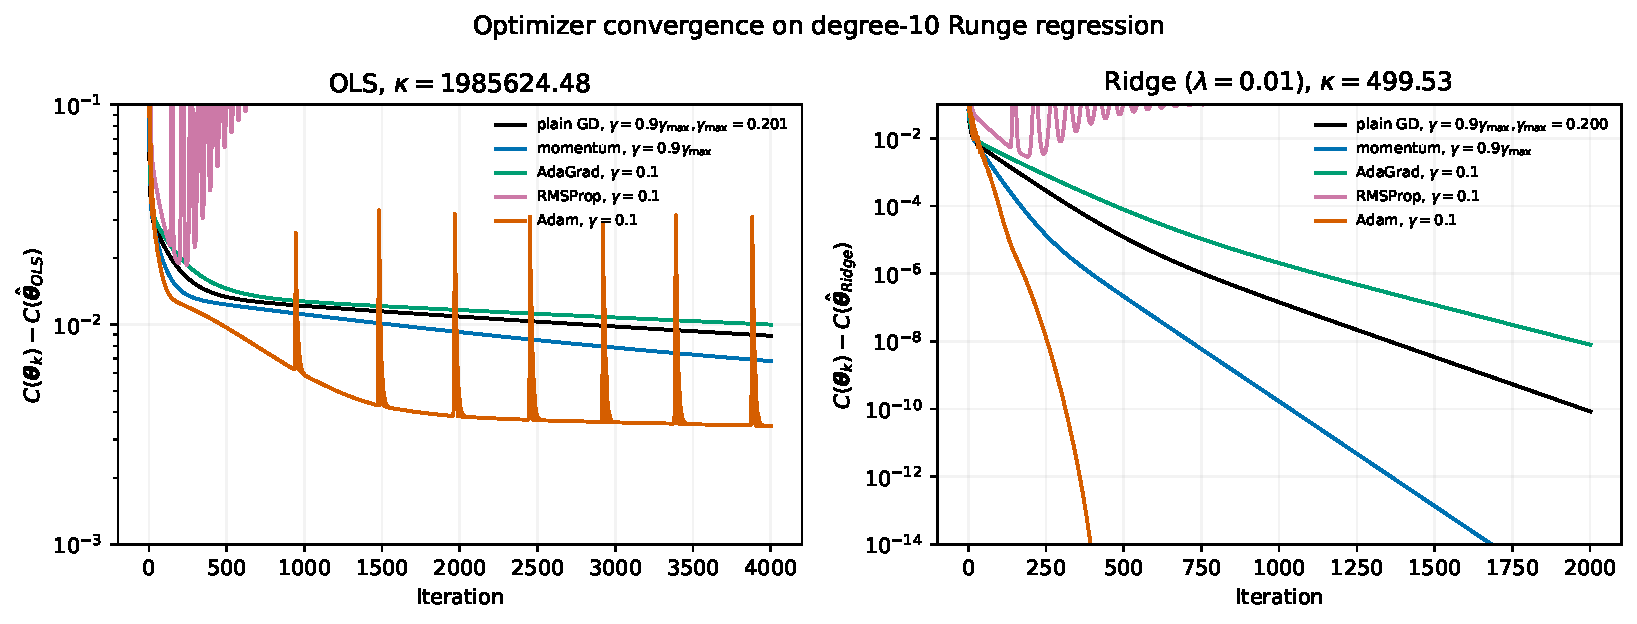
\includegraphics[width=\linewidth]{part_f_optimizer_convergence.pdf}
    \caption{Convergence of gradient descent, momentum, AdaGrad, RMSProp and Adam for degree-10 OLS and Ridge regression.}
    \label{fig:part_f_convergence}
\end{figure}

The convergence of the different optimizers described in Section~\ref{section:methods} is shown in Figure~\ref{fig:part_f_convergence}, with the same 10-degree polynomial setup as before. We see that all methods converge, apart from RMSProp that was initiliazed with a too high learning rate. Adam converges the fastest.

\begin{figure}[htbp]
    \centering
    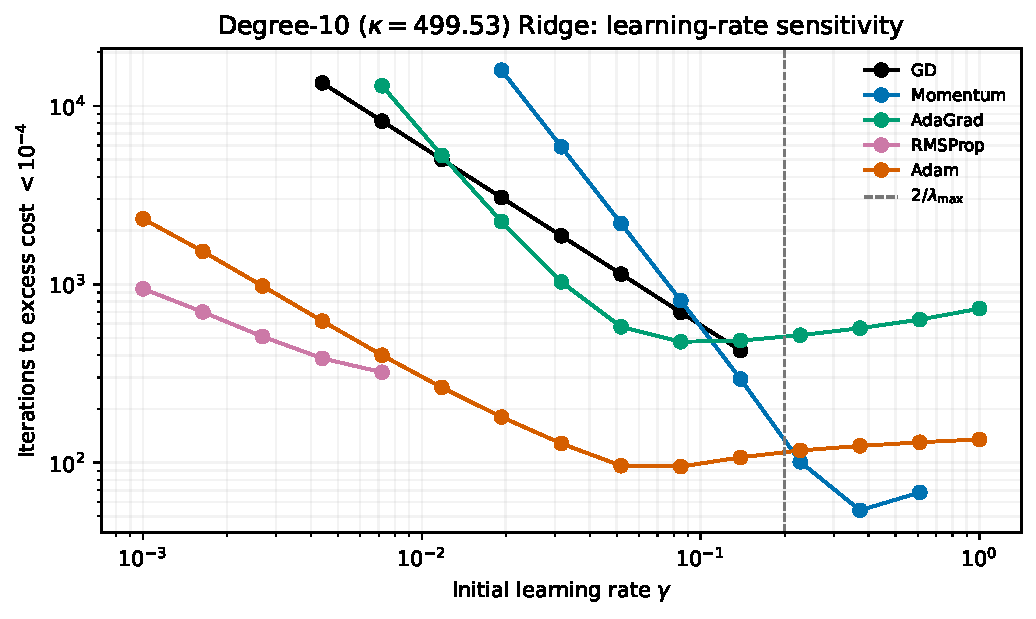
\includegraphics[width=\linewidth]{part_f_learning_rate_sensitivity.pdf}
    \caption{Iterations needed to reach an excess cost below $10^{-4}$, as a function of the learning rate $\gamma$, for degree-10 Ridge regression.}
    \label{fig:part_f_scan}
\end{figure}

Figure~\ref{fig:part_f_scan} shows that the methods differ in their sensitivity to $\gamma$, with some methods remaining stable over a wide range of learning rates while others require a more careful tuning (e.g., RMSProp). Adam is very robust, performing well over all tested range of learning rates. Momentum is also relatively robust, and also is the method that performs best at a tuned learning rate.

\begin{table}[htbp]
    \centering
    \caption{Best scanned learning rates among runs that reach the target parameter error of $10^{-4}$.}
    \label{tab:optimizer-learning-rates}
    \begin{tabular}{lrr}
        \hline\hline
        Method   & Best gamma & Iterations \\
        \hline
        GD       & 0.1389     & 425        \\
        Momentum & 0.3728     & 54         \\
        AdaGrad  & 0.08483    & 476        \\
        RMSProp  & 0.007197   & 321        \\
        Adam     & 0.08483    & 95         \\
        \hline\hline
    \end{tabular}
\end{table}


Table~\ref{tab:optimizer-learning-rates} summarizes the best-case performance of each method: momentum is the fastest at its optimal $\gamma$, needing only 54 iterations, with Adam close behind at 95 iterations. AdaGrad and plain gradient descent are the slowest, needing several hundred iterations even at their best learning rate, while RMSProp needs a much smaller $\gamma\approx0.0072$ than the others to remain stable.


\subsection{Lasso regression}

As discussed in Section~\ref{section:methods}, the $\ell_1$ penalty is not differentiable at $\theta_j=0$. When evaluating the gradient at $\boldsymbol{\theta}=\boldsymbol{0}$, JAX and our analytical implementation differ by exactly $\lambda$ in each coordinate. This is because JAX returns $+1$ as the subgradient of $|\theta_j|$ at zero, while our implementation uses {\texttt{np.sign(0) = 0}}. We therefore see in Eq.~\eqref{eq:gradient_lasso} why the gradient at zero differs by $\lambda$. Both choices are valid subgradients.

\begin{table}[htbp]
    \centering
    \caption{Lasso regression with some selected optimizers, compared with Sklearn's Lasso.}
    \label{tab:lasso-optimizers}
\begin{tabular}{lrrr}
\hline\hline
Optimizer & Iterations & Final cost & $\|\theta-\theta_{\mathrm{sklearn}}\|_2$ \\
\hline
GD ($\gamma=0.01$) & 30000 & 0.04504 & 0.0008636 \\
Momentum ($\gamma=0.01$) & 30000 & 0.04608 & 0.3122 \\
Adam ($\gamma=0.01$) & 30000 & 0.04511 & 0.004622 \\
\hline\hline
\end{tabular}
\end{table}


Table~\ref{tab:lasso-optimizers} compares gradient descent, momentum and Adam against Scikit-learn's \texttt{Lasso} after 30~000 iterations at $\gamma=0.01$. Gradient descent and Adam give solutions close to the reference solution, with distances of $8.6\times10^{-4}$ and $4.6\times10^{-3}$. Momentum is further from the reference solution, with a distance of $0.31$.


\begin{table}[htbp]
    \centering
    \caption{Lasso coefficient estimates for selected polynomial degrees.}
    \label{tab:lasso-theta}
    \begin{tabular}{rrr}
        \hline\hline
        Degree & Exact zeros & $|\theta| < 10^{-3}$ \\
        \hline
        2      & 0           & 0                    \\
        6      & 0           & 2                    \\
        8      & 0           & 0                    \\
        10     & 0           & 2                    \\
        12     & 0           & 3                    \\
        15     & 0           & 4                    \\
        \hline\hline
    \end{tabular}
\end{table}


Table~\ref{tab:lasso-theta} counts, for a few polynomial degrees, how many fitted coefficients are exactly zero versus only close to zero ($|\theta_j|<10^{-3}$). None of our fits produce exact zeros, although several coefficients are driven very close to zero at higher degrees. This is related to how we handle the subgradient at zero. The updates approach zero but do not explicitly set coefficients to zero, in contrast to Scikit-learn, which uses coordinate descent for Lasso \cite{scikitlasso}, and can set coefficients exactly to zero \cite{lecturebook}.

\begin{figure}[htbp]
    \centering
    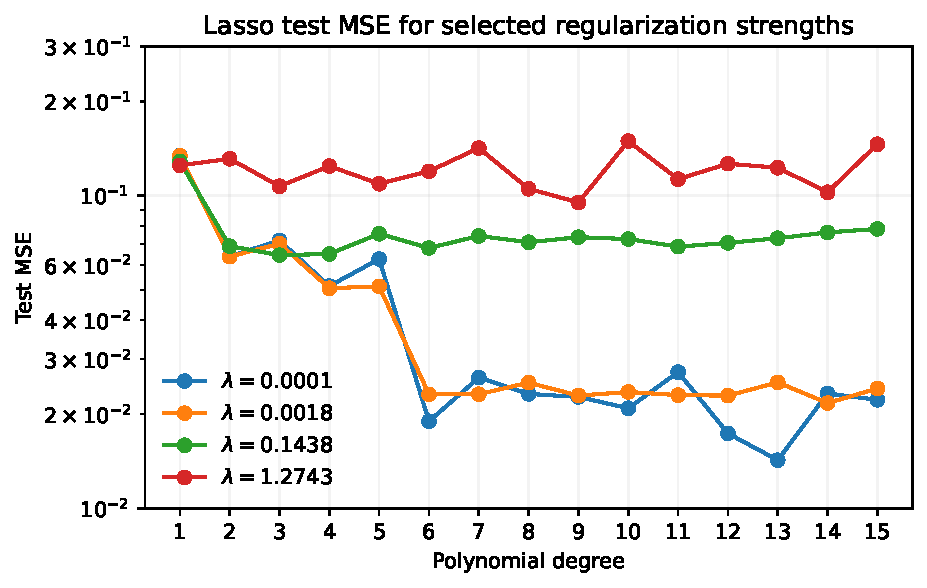
\includegraphics[width=\linewidth]{part_g_lasso_selected_lambda.pdf}
    \caption{Lasso test MSE as a function of polynomial degree for four values of $\lambda$, fitted with Adam.}
    \label{fig:part_g_curves}
\end{figure}

Figure~\ref{fig:part_g_curves} shows the same behaviour as Ridge in Fig.~\ref{fig:part_b_curves}, where the curves become flatter as the penalty increases.

\subsection{Stochastic gradient descent}

\begin{figure}[htbp]
    \centering
    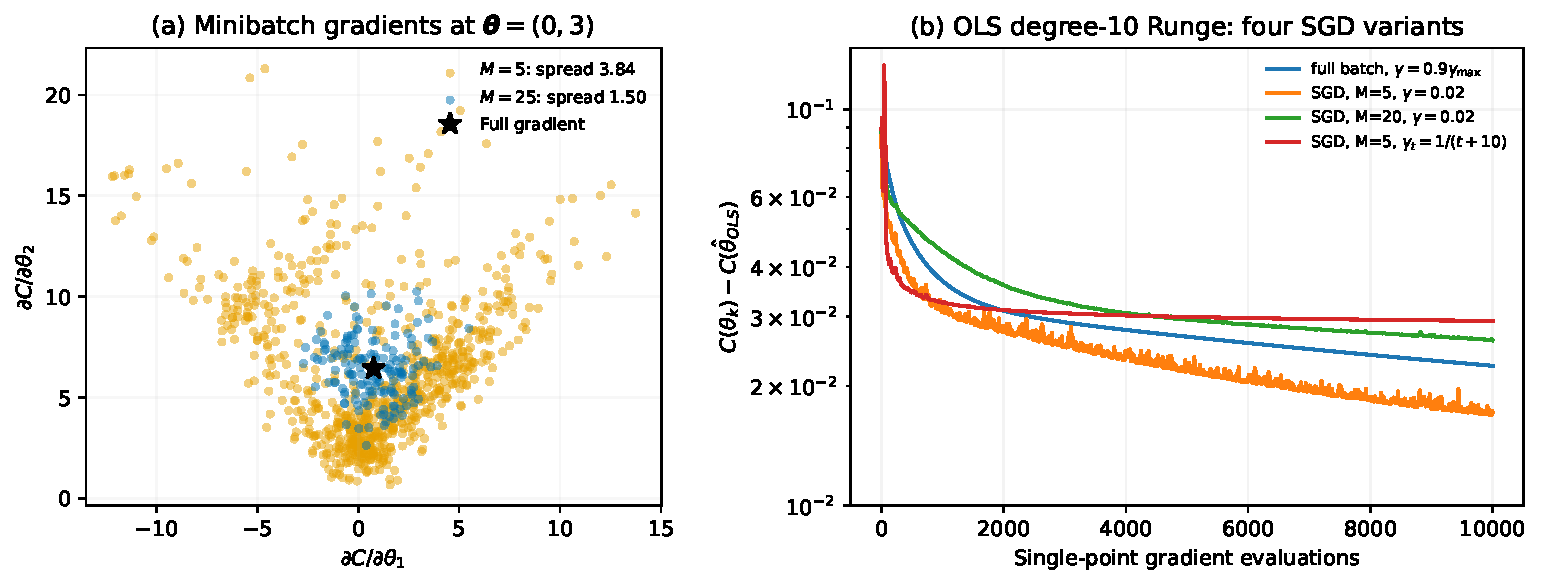
\includegraphics[width=\linewidth]{part_h_sgd.pdf}
    \caption{(a) Minibatch gradients of a degree-2 OLS problem at a fixed $\boldsymbol{\theta}$, for batch sizes $M=5$ and $M=25$, compared with the full gradient. (b) Distance to the closed-form OLS solution for four plain SGD variants on the degree-10 problem. 100 epochs.}
    \label{fig:part_h}
\end{figure}

Figure~\ref{fig:part_h}(a) shows the variations in the minibatch gradients around the full gradient. The measured spread decreases from $3.84$ for $M=5$ to $1.50$ for $M=25$. This is close to the expected $1/\sqrt{M}$ scaling mentioned in Section~\ref{section:methods}: increasing the batch size from $M=5$ to $M=25$ should multiply the standard deviation by $1/\sqrt{5}\approx0.45$. As seen in the figure, the larger batch therefore gives a tighter estimate of the full gradient.

Figure~\ref{fig:part_h}(b) shows that, per single-point gradient evaluation, the SGD variants start with faster convergence than full-batch gradient descent, but most eventually converge more slowly due to noise in the updates and reach a plateau. Even the decaying learning-rate variant eventually slows down and reaches a plateau. Interestingly, SGD with batch size $M=5$ performs best, reaching the lowest distance to the closed-form solution within the 100 epochs, even beating full-batch gradient descent. The learning rates were chosen based on a few initial experiments and were not finely tuned, so the results could likely be improved with further tuning.

\subsection{Final comparison}

\begin{figure}[htbp]
    \centering
    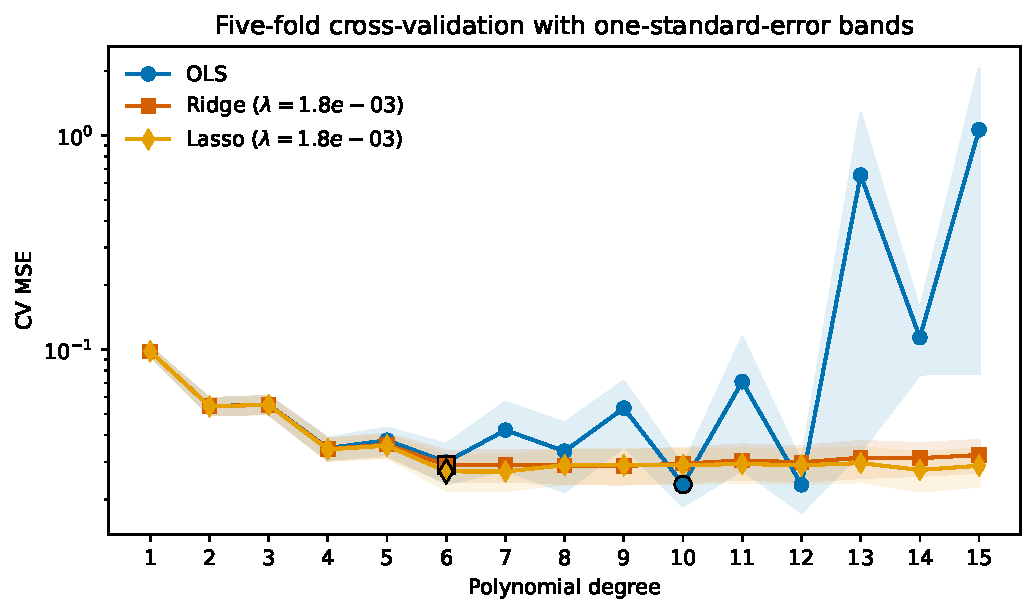
\includegraphics[width=\linewidth]{part_i_final_cv_comparison.pdf}
    \caption{Five-fold cross-validation MSE, with one-standard-error bands, for OLS as a function of degree and for Ridge and Lasso at their selected $\lambda$. Markers show the degree chosen by the one-standard-error rule.}
    \label{fig:part_i}
\end{figure}

\begin{table}[htbp]
    \centering
    \caption{Final OLS, Ridge and Lasso models selected using five-fold cross-validation.}
    \label{tab:final-models}
\begin{tabular}{lrlrrrr}
\hline\hline
Model & Degree & Lambda & CV MSE & CV SE & Test MSE & Test R2 \\
\hline
OLS & 10 & - & 0.0235 & 0.00485 & 0.03702 & 0.7017 \\
Ridge & 6 & 1.8e-03 & 0.02895 & 0.004678 & 0.03174 & 0.7442 \\
Lasso & 6 & 1.8e-03 & 0.02704 & 0.004996 & 0.02323 & 0.8128 \\
\hline\hline
\end{tabular}
\end{table}


The final comparison is shown in Fig.~\ref{fig:part_i} and Table~\ref{tab:final-models}. The models were selected using five-fold cross-validation and the one-standard-error rule, and were then evaluated once on the untouched test set.

The CV curves show that regularization makes the test error less sensitive to the polynomial degree. Both Ridge and Lasso have very flat curves from about degree 6 to 15, while the OLS curve increases and fluctuates at the higher degrees, similar to what was observed earlier. The Ridge and Lasso curves are also very similar, with narrow standard-error bands, compared to OLS that have wider bands as the degree increases.

The one-standard-error rule selects degree 10 for OLS and degree 6 for both regularized models. On the untouched test set, OLS obtains a test MSE of $0.0370$ and $R^2=0.702$, while Ridge with $\lambda\approx1.8\times10^{-3}$ gives $R^2=0.744$. Lasso selects a similar $\lambda$ and gives the lowest test error, with $R^2=0.813$.

The degree-12 OLS model found in the test-error scan in Fig.~\ref{fig:part_a_mse_r2} has a higher test $R^2$ (about $0.8473$) than the degree-10 model selected here. This is expected since degree 12 was chosen based on the test set itself. However, using the test set to select the degree would make the final test performance optimistic. In this final comparison, the test set is kept untouched and the degree is selected using cross-validation on the training data.

Both regularized models perform better than OLS, even though OLS has the lowest CV MSE. This is consistent with the earlier results: at higher degrees, OLS becomes more sensitive to the training data, and regularization reduces this sensitivity. Ridge and Lasso do this in different ways, and Lasso gives the best result for this particular split. The $\ell_1$ penalty also shrinks some coefficients more strongly towards zero, although none of the coefficients in our final Lasso model are exactly zero.

\section{Conclusion}\label{section:conclusion}
We have fitted polynomial models of up to degree 15 to a noisy sample of Runge's function using OLS, Ridge and Lasso regression, together with bootstrap resampling, cross-validation and several gradient-based optimization methods. The OLS results showed that increasing the polynomial degree initially reduces bias, but eventually leads to unstable coefficients and increasing variance. The bias-variance decomposition showed this trade-off. Ridge and Lasso reduced the sensitivity to the training data, and both outperformed OLS in the final test comparison, with $R^2=0.744$ and $0.813$ respectively, compared with $0.702$ for OLS.

The optimization experiments showed that the closed-form solutions for OLS and Ridge can be reproduced with iterative methods, but that their convergence rates depend strongly on the optimizer, learning rate and conditioning of the problem. Momentum gave the fastest convergence among the tested optimizers, after tuning its learning rate, while the adaptive methods (apart from RMSProp) were less sensitive to the learning-rate choice. For SGD, smaller batches gave noisier gradient estimates but allowed more parameter updates for the same number of gradient evaluations. The Lasso experiments also showed a limitation of our subgradient approach: the fitted coefficients could become very small, but were not driven to exactly zero.

There are several possible extensions. The most direct improvement would be to implement Lasso using coordinate descent, which is also the method used by Scikit-learn, and can produce exact zero coefficients. It would be interesting to see whether this changes the fitted model and its prediction performance. Since our final results are based on one train-test split, repeating the comparison with different splits would also show how much the reported test performance depends on the particular split. This could give a clearer picture of how stable the difference between OLS, Ridge and Lasso is.

\bibliography{biblio}

\onecolumngrid
\newpage

\section{Appendix}
\appendix
\section{Use of AI/LLM tools}
\subsection{Tools used}
\begin{itemize}
    \item GitHub Copilot (VS Code, throughout) for code autocompletion
    \item ChatGPT (chatgpt.com, September-October 2026) for grammar corrections, rephrasing, and improving the fluency and clarity of the text. ALL ideas, analysis, structure are our own. ChatGPT was also used to assist with some code (mentioned below).
\end{itemize}

\subsection{Text writing and editing.}
\begin{tabular}{llp{7cm}}
    Section          & Level & Notes                                           \\ \hline
    Abstract         & 1-2   & some rephrasing and language corrections        \\
    Introduction     & 2     & rephrased for clarity; ideas and structure ours \\
    Theory / Methods & 2     & rephrased for clarity; ideas and structure ours \\
    Results          & 2     & rephrased for clarity; ideas and structure ours \\
    Conclusion       & 2     & rephrased for clarity; ideas and structure ours \\
\end{tabular}

\subsection{Code generation and assistance.}

\begin{tabular}{llp{7cm}}
    Folder/file                                & Level & Description                                                                                                                                                                                                                          \\ \hline
    \texttt{models/}                           & 1     & Copilot autocomplete only                                                                                                                                                                                                            \\
    \texttt{optimizers/}                       & 1     & Copilot autocomplete only                                                                                                                                                                                                            \\
    \texttt{resampling/}                       & 1     & Copilot autocomplete only                                                                                                                                                                                                            \\
    \texttt{scripts/part\_a.py-part\_h.py}     & 1     & Copilot autocomplete only                                                                                                                                                                                                            \\
    \texttt{scripts/part\_i.py}                & 2     & ChatGPT assisted with the one-standard-error degree selection logic                                                                                                                                                                  \\
    \texttt{utils/} (excl. \texttt{report.py}) & 1     & Copilot autocomplete only                                                                                                                                                                                                            \\
    \texttt{utils/report.py}                   & 2-3   & Copilot generated the \texttt{save\_latex\_table} function; I modified to use \texttt{hline} instead of top/mid/bottomrule. Simple prompt where I asked it to generate.                                                              \\
    \texttt{model\_fitter.py}                  & 1     & Copilot autocomplete only                                                                                                                                                                                                            \\
    \texttt{notebooks/Project1\_results.ipynb} & 2-3   & ChatGPT helped with the coefficient masking/axis-limit logic and generated the coefficient heatmap. Simple prompt where I asked it to generate.                                                                                      \\
    \\
    \texttt{README.md}                         & 3-4   & Github Copilot generated the content and structure of the README file.  I pasted in a README file from another project, and asked it to imitate its structure. The rest of the prompt can be found at the bottom of the README file. \\
\end{tabular}

\end{document}
